\subsubsection{Procedure}\label{procedureVerifica}
\subsubsubsection{Approvazione di un ticket}
La procedura di approvazione di un ticket segue il diagramma di attività riportato in \customRef{fig:rigetto_approvazioneTicket}{figura}.
L'attività di chiusura di ticket è delegata al \rV, che:
\begin{enumerate}
\item Riceve la notifica di un ticket con stato ``Resolved'';
\item Effettua una ricerca approfondita per trovare eventuali anomalie ancora presenti, che dà esito negativo;
\item Imposta lo stato del ticket ad ``Approved'';
\item Imposta lo stato del ticket di verifica a ``Resolved''.
\end{enumerate}
\subsubsubsection{Rigetto di un ticket}
La procedura di rigetto di un ticket da parte del \rV segue il diagramma di attività riportato in \customRef{fig:rigetto_approvazioneTicket}{figura}.
Il \rV:
\begin{enumerate}
\item Riceve la notifica di un ticket con stato ``Resolved'';
\item Effettua una ricerca approfondita per trovare eventuali anomalie ancora presenti, che dà esito positivo;
\item Imposta lo stato del ticket a ``Rejected'';
\item Crea una lista con le anomalie trovate;
\item Invia la lista con le anomalie al \rRP;
\item Imposta lo stato del ticket di verifica a ``Resolved''.
\end{enumerate}
\subsubsubsection{Gestione delle anomalie}\label{procGestioneAnomalie}
Al termine di un ticket, il \rV dovrà procedere alla verifica del lavoro completato. Qualora individuasse delle anomalie, dovrà registrarle nella ``\emph{lista delle anomalie}'', per consentirne la correzione tramite l'uso di una tecnica di ispezione mirata. Al termine dell’attività di verifica, se sono state individuate anomalie, il \rRP dovrà aprire dei ticket per consentirne la risoluzione e la successiva verifica.
\begin{figure}[H]
\centering
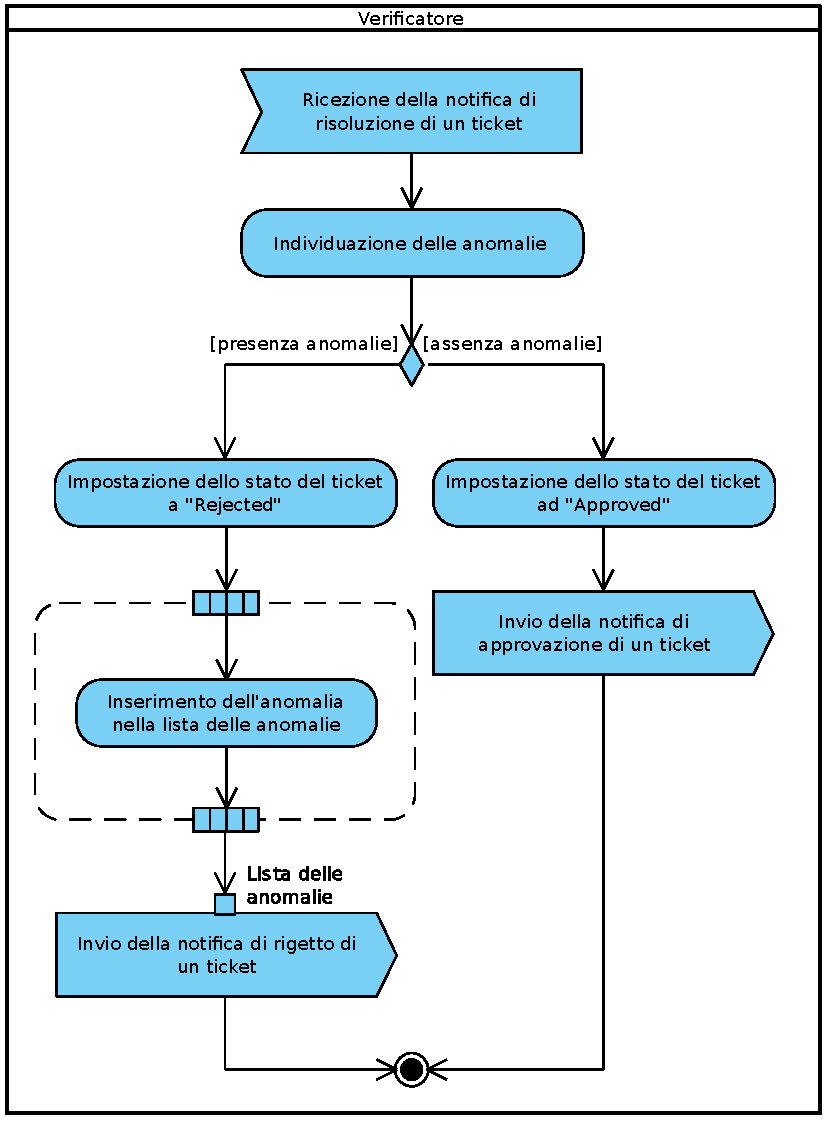
\includegraphics[width=9cm]{../immagini/rigetto_approvazioneTicket.pdf}
\caption{Diagramma di attività - rigetto/approvazione di un ticket}
\label{fig:rigetto_approvazioneTicket}
\end{figure}
